\chapter{Modelo de datos}
\label{cap:modelo}
En este capitulo se mostrará el diseño de datos lógico y físico generado para el proyecto que estamos presentando, correspondiente a la reestructuración del sistema actual. 

El modelo de datos lógico diseñado, muestra la reestructuración de la base de datos de información que se realizó en la institución financiera. 
Como lo mencionamos en el presente trabajo, la institución contaba con muchas fuentes de datos que hacian muy complicado el manejo de información
así como el gobierno de datos. 

El diseño del modelo se basó en identificar las entidades principales como socios, cuentas, transacciones y créditos para centralizar 
toda la información de los diferentes sistemas además de tener una fuente de datos para la generación de los reportes de las diferentes áreas.

En la siguiente imagen se muestra el diseño lógico generado.

\section{Modelo de datos lógico}
\begin{figure}[htb]
  \begin{center}
    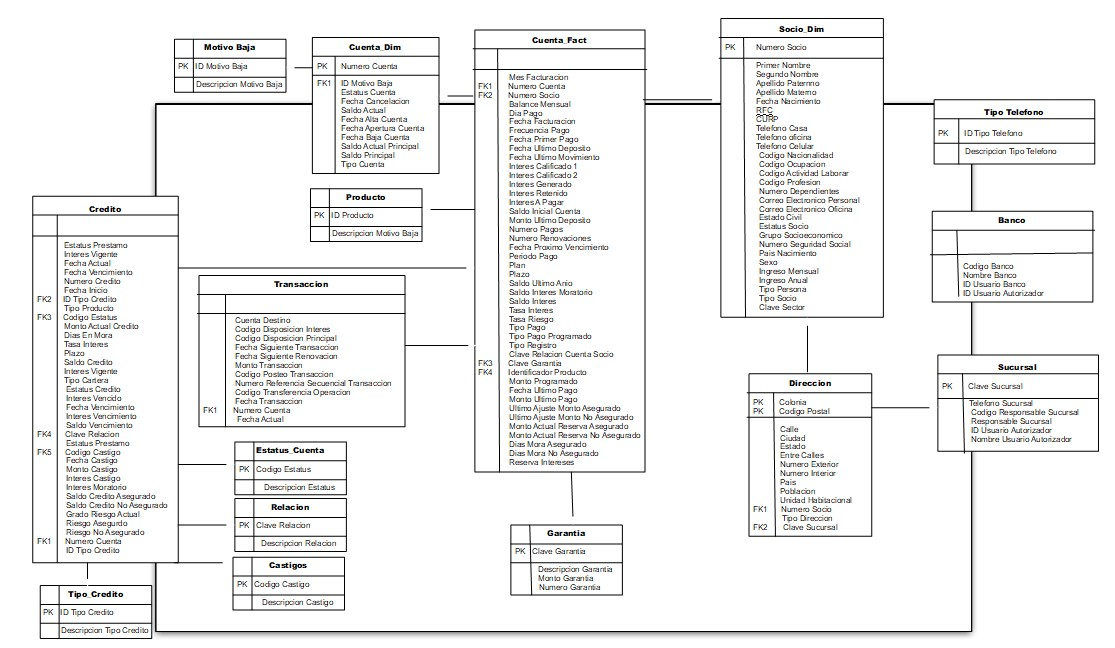
\includegraphics[width=\linewidth]{Modelo_logico.jpg}
        \caption{Modelo lógico de la base de datos.}
    \label{fig:modelo-logico}
  \end{center}
\end{figure}


\section{Modelo de datos físico}

Una vez generado el modelo de datos lógico, se procedió a diseñar el modelo de datos físico que se implementó a nivel base de datos.

Este modelo se presenta en la siguiente imagen:

\section{Modelo de datos físico}
\begin{figure}[htb]
  \begin{center}
    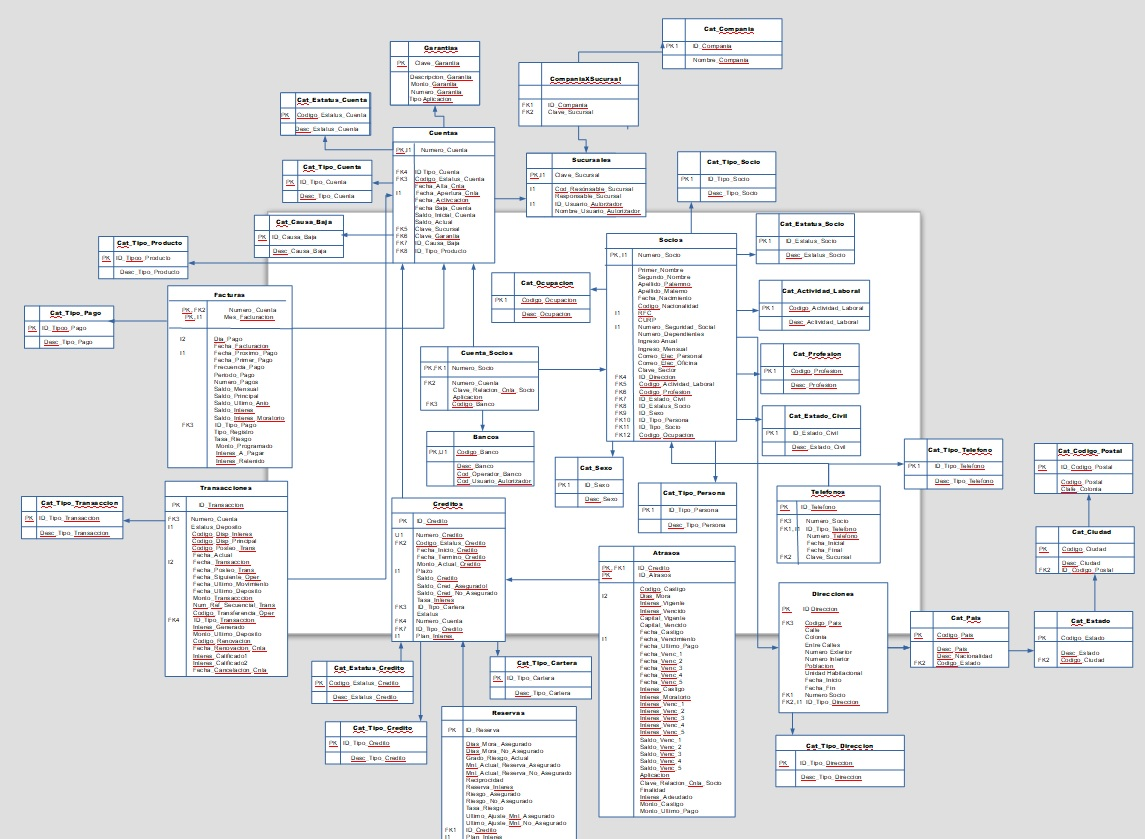
\includegraphics[width=\linewidth]{Modelo_fisico.jpg}
        \caption{Modelo físico de la base de datos.}
    \label{fig:modelo-fisico}
  \end{center}
\end{figure}

\cleardoublepage

%%% Local Variables:
%%% TeX-master: "Tesis"
%%% End:
